\documentclass[20pt,a4paper]{extarticle}
\usepackage[utf8]{inputenc}
\usepackage[english]{babel}

\usepackage{amsmath}
\usepackage{amsfonts}
\usepackage{amssymb}
\usepackage{mathtools}
\usepackage{systeme}
\sysdelim..

\usepackage{graphicx}
\usepackage{caption}
\usepackage{subcaption}
\usepackage{lmodern}
\usepackage{tikz}
\usetikzlibrary{calc}
\usepackage{titlesec}
\usepackage{environ}
\usepackage{xcolor}
\usepackage{fancyhdr}
\usepackage[colorlinks = true, linkcolor = black]{hyperref}
\usepackage{xparse}
\usepackage{enumitem}
\usepackage{comment}
\usepackage{wrapfig}
\usepackage{soul}
\usepackage[capitalise]{cleveref}

\usepackage[left=2cm,right=2cm,top=2cm,bottom=2cm]{geometry}
\usepackage{multicol}
\usepackage[indent=0pt]{parskip}

\newcommand{\spaceP}{\vspace*{0.5cm}}
\newcommand{\Span}{\mathrm{Span}\,}
\newcommand{\range}{\mathrm{range}\,}
\newcommand{\ra}{\rightarrow}
\newcommand{\curl}{\mathrm{curl} \,}
\newcommand{\hint}[1]{\scalebox{2}{$\displaystyle\int_{\scalebox{0.35}{$#1$}}$}\,}
\newcommand{\hiint}[1]{\scalebox{2}{$\displaystyle\iint_{\scalebox{0.35}{$#1$}}$}\,}
\newcommand{\hiiint}[1]{\scalebox{2}{$\displaystyle\iiint_{\scalebox{0.35}{$#1$}}$}\,}
\renewcommand{\div}{\mathrm{div}\,}

\makeatletter
\renewcommand*\env@matrix[1][*\c@MaxMatrixCols c]{%
  \hskip -\arraycolsep
  \let\@ifnextchar\new@ifnextchar
  \array{#1}}
\makeatother

%% Redefining sections
\newcommand{\sectionformat}[1]{%
    \begin{tikzpicture}[baseline=(title.base)]
        \node[rectangle, draw] (title) {#1};
    \end{tikzpicture}
    
    \noindent\hrulefill
}

\newif\ifhNotes 

\hNotesfalse

\ifhNotes
	\newcommand{\hideNotes}[1]{%
	\phantom{#1}
	}
	\newcommand{\hideNotesU}[1]{%
	\underline{\hspace{1mm}\phantom{#1}\hspace{1mm}}
	}
\else
	\newcommand{\hideNotes}[1]{#1}
	\newcommand{\hideNotesU}[1]{\textcolor{blue}{#1}}
\fi

% default values copied from titlesec documentation page 23
% parameters of \titleformat command are explained on page 4
\titleformat%
    {\section}% <command> is the sectioning command to be redefined, i. e., \part, \chapter, \section, \subsection, \subsubsection, \paragraph or \subparagraph.
    {\normalfont\large\scshape}% <format>
    {}% <label> the number
    {0em}% <sep> length. horizontal separation between label and title body
    {\centering\sectionformat}% code preceding the title body  (title body is taken as argument)

%% Set counters for sections to none
\setcounter{secnumdepth}{0}

%% Set the footer/headers
\pagestyle{fancy}
\fancyhf{}
\renewcommand{\headrulewidth}{0pt}
\renewcommand{\footrulewidth}{2pt}
\lfoot{P.-O. Paris{\'e}}
\cfoot{MATH 311}
\rfoot{Page \thepage}

%% Defining example environment
\newcounter{example}[section]
\NewEnviron{example}%
	{%
	\noindent\refstepcounter{example}\fcolorbox{gray!40}{gray!40}{\textsc{\textcolor{red}{Example~\theexample.}}}%
	%\fcolorbox{black}{white}%
		{  %\parbox{0.95\textwidth}%
			{
			\BODY
			}%
		}%
	}

\newcounter{theorem}
\NewEnviron{theorem}%
	{%
	\noindent\refstepcounter{theorem}\fcolorbox{gray!40}{gray!40}{\textsc{\textcolor{black}{Theorem~\thetheorem.}}}%
	%\fcolorbox{black}{white}%
		{  %\parbox{0.95\textwidth}%
			{
			\BODY
			}%
		}%
	}

\newcounter{definition}[section]
\NewEnviron{definition}%
	{%
	\noindent\refstepcounter{definition}\fcolorbox{gray!40}{gray!40}{\textsc{\textcolor{black}{Definition~\thedefinition.}}}%
	%\fcolorbox{black}{white}%
		{  %\parbox{0.95\textwidth}%
			{
			\BODY
			}%
		}%
	}

\NewEnviron{algorithm}
	{%
	\noindent\refstepcounter{definition}\fcolorbox{gray!40}{gray!40}{\textsc{\textcolor{black}{Algorithm~\thedefinition.}}}%
	%\fcolorbox{black}{white}%
		{  %\parbox{0.95\textwidth}%
			{
			\BODY
			}%
		}%
	}

\NewEnviron{solution}%
	{%
	\noindent \fcolorbox{gray!40}{gray!40}{\textsc{\textcolor{blue}{Solution.}}}%
	%\fcolorbox{black}{white}%
		{  %\parbox{0.95\textwidth}%
			{
			%\textcolor{blue}
			}%
		}%
	}

\NewEnviron{proof}%
	{%
	\noindent \fcolorbox{gray!40}{gray!40}{\textsc{\textcolor{blue}{Proof.}}}%
	%\fcolorbox{black}{white}%
		{  %\parbox{0.95\textwidth}%
			{
			\textcolor{blue}{%
			\BODY
			}
			}%
		}%
	}
%%% Ignorer les notes
%\excludecomment{notes}

%%%%
\begin{document}
\thispagestyle{empty}

\begin{center}
\vspace*{2.5cm}

{\Huge \textsc{Math 311}}

\vspace*{1.5cm}

{\LARGE \textsc{Chapter 2}} 

\vspace*{0.75cm}

\noindent\textsc{Section 2.2: Matrix-Vector Multiplication}

\vspace*{0.75cm}

\tableofcontents

\vfill

\noindent \textsc{Created by: Pierre-Olivier Paris{\'e}} \\
\textsc{Spring 2024}
\end{center}

\newpage

\section{Matrix-Vector Multiplication}

\begin{example}
Write the system
	\[
		\systeme{3x_1 + 2x_2 - 4x_3 = 0, x_1 - 3x_2 + x_3 = 3, x_2 - 5x_3 = -1}
	\]
in a compact form using a linear combination of vectors.
\end{example}

\begin{solution}

\end{solution}

\vfill 

\underline{Note:} Any system of linear equations can be rewritten as $A \mathbf{x} = \mathbf{b}$, where $A$ is the matrix of coefficients, $\mathbf{x}$ is the $n$-vector containing the unknown, and $\mathbf{b}$ is the $m$-vector containing the constant terms of each equation.

\newpage 

\begin{definition}
	\begin{itemize}
	\item Let $A = [\mathbf{a_1} \,\, \mathbf{a_2} \, \, \cdots \, \, \mathbf{a_n} ]$ be an $m \times n$ matrix, where the $m$-vectors $\mathbf{a_1}$, $\mathbf{a_2}$, $\ldots$, $\mathbf{a_n}$ represent the columns. 
	\item Let $\mathbf{x}$ be any $n$-vector. 
	\end{itemize}
The \textbf{product} $A \mathbf{x}$ is defined to be the $m$-vector:
	\[
		A \mathbf{x} = x_1 \mathbf{a_1} + x_2 \mathbf{a_2} + \cdots + x_n \mathbf{a_n} .
	\]
\end{definition}

\begin{example}\label{Example:MatrixVectorProduct}
If $A = \begin{bmatrix} 2 & -1 & 3 & 5 \\ 0 & 2 & -3 & 1 \\ -3 & 4 & 1 & 2 \end{bmatrix}$ and $\mathbf{x} = \begin{bmatrix} 2 \\ 1 \\ 0 \\ -2 \end{bmatrix}$, then compute $A \mathbf{x}$.
\end{example}

\begin{solution}

\end{solution}

\newpage 

Properties:
	\begin{itemize}
		\item $A (\mathbf{x} + \mathbf{y}) = A \mathbf{x} + A \mathbf{y}$.
		\item $A (a\mathbf{x}) = a (A\mathbf{x}) = (aA) \mathbf{x}$, for any scalar $a$.
		\item $(A + B) \mathbf{x} = A\mathbf{x} + B \mathbf{y}$.
	\end{itemize}


\section{The Dot Product}

\begin{definition}
If $\mathbf{x}$ is an $1 \times n$ vector and $\mathbf{y}$ is an $n \times 1$ vectors, their \textbf{dot product} is defined to be the number
	\[
		\mathbf{x} \cdot \mathbf{y} := x_1 y_1 + x_2 y_2 + \ldots + x_n y_n .
	\]
\end{definition}

\begin{example}
Use the dot product to compute $A \mathbf{x}$ where $A$ and $\mathbf{x}$ are as in Example \ref{Example:MatrixVectorProduct}.
\end{example}

\begin{solution}

\end{solution}

\newpage 

\phantom{2} 

\vfill 

\underline{The Dot Product Rule.}

\begin{minipage}{0.45\textwidth}
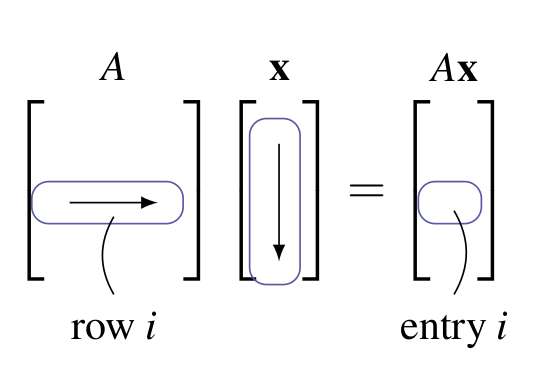
\includegraphics[scale=0.4]{DotProductRule.png}
\end{minipage}
\hspace*{1cm}
\begin{minipage}{0.45\textwidth}
To obtain the entry $i$ of $A \mathbf{x}$, take the dot product of row $i$ of $A$ with the vector $\mathbf{x}$.
\end{minipage}

\newpage 

\begin{example}
Find an $n \times n$ matrix $A$ such that $A \mathbf{x} = \mathbf{x}$, for any $\mathbf{x} \in \mathbb{R}^n$.
\end{example}

\begin{solution}

\end{solution}

\vfill 

\begin{theorem}
Let $A$ and $B$ be two $m \times n$ matrices. \\ 
If $A \mathbf{x} = B \mathbf{x}$ for any $\mathbf{x} \in \mathbb{R}^n$, then $A = B$. 
\end{theorem}

\newpage 

\section{Transformations}

\begin{example}
A function is defined as follows: it reflects a $2 \times 1$ vector accross the $x$-axis in the 2D space. Illustrate graphically the \textbf{action} of this function and find a formula to describe it.
\end{example}

\begin{solution}

\end{solution}

\newpage

\begin{definition}
Given an $m \times n$ matrix $A$, the \textbf{matrix transformation induced} by the matrix $A$ denoted by $T_A$ is defined by
	\[
		T_A (\mathbf{x} ) = A \mathbf{x} \quad \forall \mathbf{x} \in \mathbb{R}^n .
	\]
\end{definition}

\underline{Note:}
	\begin{itemize}
		\item For each $\mathbf{x} \in \mathbb{R}^n$, we have $T_A (\mathbf{x}) \in \mathbb{R}^m$. In this case, the expression of $T_A (\mathbf{x})$ is called the \textbf{action} of $T_A$.
		\item Therefore, $T_A : \mathbb{R}^n \ra \mathbb{R}^m$ is a function. 
		\item For two matrices $A$ and $B$, we say that $T_A$ and $T_B$ are \textbf{equal} if they have the same action, meaning $T_A (\mathbf{x}) = T_B (\mathbf{x})$, for any $\mathbf{x} \in \mathbb{R}^n$.
	\end{itemize}


\begin{example}
Let $A$ be the $m \times n$ zero matrix. Then $T_A$ is called the \textbf{zero matrix-transformation}. Show that $T_A (\mathbf{x}) = \mathbf{0}$, where $\mathbf{0}$ is the $m$-vector with $0$ in all its entries.
\end{example}

\begin{solution}

\end{solution}





\end{document}